\documentclass[11pt]{article}

\usepackage[utf8]{inputenc}
\usepackage[T1]{fontenc}
\usepackage{mathptmx}
% \usepackage[skip=3em]{caption}

\topmargin -4em
\setlength{\textwidth} {420pt}
\setlength{\textheight} {620pt}
\setlength{\oddsidemargin} {20pt}
\setlength{\marginparwidth} {72in}


\usepackage{fancyhdr}
\usepackage{hyperref}
\usepackage{graphicx}
\usepackage{subcaption}
\usepackage{mathtools}

% may not work with travis ci
\usepackage{color}

% Use elastic spacing around the headers
\usepackage{titlesec}
\titlespacing\section{0pt}{6pt plus 4pt minus 2pt}{4pt plus 2pt minus 2pt}

% set it so that subsubsections have numbers and they
% are displayed in the TOC (maybe hard to read, might want to disable)
\setcounter{secnumdepth}{3}
\setcounter{tocdepth}{3}

% define widow protection
\def\widow#1{\vskip #1\vbadness10000\penalty-200\vskip-#1}

\clubpenalty=10000  % Don't allow orphans
\widowpenalty=10000 % Don't allow widows

% this should give you the ability to use some math symbols that
% were available by default in standard latex (i.e. \Box)
\usepackage{latexsym}

% define a little section heading that doesn't go with any number
\def\littlesection#1{
  \widow{2cm}
  \vskip 0.5cm
  \noindent{\bf #1}
  \vskip 0.0001cm
}

\pagestyle{fancyplain}

\newcommand{\tstamp}{\today}


% \renewcommand{\sectionmark}[1]{\markright{#1}}
% \lhead[\Section \thesection]            {\fancyplain{}{\rightmark}}
% \chead[\fancyplain{}{}]                 {\fancyplain{}{}}
% \rhead[\fancyplain{}{\rightmark}]       {\fancyplain{}{\thepage}}
% \cfoot[\fancyplain{\thepage}{}]         {\fancyplain{\thepage}{}}
%
% \newlength{\myVSpace}% the height of the box
% \setlength{\myVSpace}{1ex}% the default,
% \newcommand\xstrut{\raisebox{-.5\myVSpace}% symmetric behaviour,
%   {\rule{0pt}{\myVSpace}}%
% }

% leave things with no spacing extra spacing in the final version of the paper
\renewcommand{\baselinestretch}{1.0} % must go before the begin of doc

% suppress the use of indentation for a paragraph
\setlength{\parindent}{0.0in}
\setlength{\parskip}{0.1in}


% custom commands
\newcommand{\name}{{\sc RayTerm}}
\newcommand{\rayorg}{\vec{R_{origin}}}
\newcommand{\raydir}{\vec{R_{direction}}}

\newcommand\todo[1]{
\begin{center}
  \color{red}
  {\bf TODO}\\
  #1
\end{center}
}

% begin actual document

\begin{document}

% handle widows appropriately
\def\widow#1{\vskip #1\vbadness10000\penalty-200\vskip-#1}

% make the title section

\thispagestyle{empty}
\begin{center}
  {\Huge
    \name
    \par
  }
  {\LARGE
    A Ray-Tracing Rendering Engine for XTerm-like Terminals
    \par
  }
  {\normalsize
    Saejin Mahlau-Heinert \\
    Department of Computer Science \\
    Allegheny College \\
    {\tt mahlauheinerts@allegheny.edu} \\
    \url{https://saejinmh.com} \\
    \vspace*{.1in} \today \\ \vspace*{.1in}
    \par
  }
  \vskip 2em
\end{center}

% Default "abstract" environment is too small; customize one instead:
\begin{center}
  \large\bf Abstract
  \vspace{-1em}
\end{center}

\begin{quote}

Over the many years of innovation in the field of computer graphics, advances in rendering have led to massive increases in the fidelity of engaging, satisfying, and realistic computer visualizations.
\name\ is a new and unique entry into the ranks of rendering engines, and makes its own contributions to the field of computer graphics.
While harkening back to the retro aesthetics of the seventies and eighties, \name\ embraces new advances in computing power to bring fully ray-traced visuals to an old screen -- the terminal.
Using Unicode block characters to simulate pixels and a ray-tracer written in C++, a fully three dimensional scene can be rendered, complete with lighting, shadows, and physically-based materials.
\name\ can be used as an engine for terminal-based 3D tools, visualizations, games, and more; it will be fully open-source and ready for integration into other projects.

\end{quote}

\section{Introduction}
\label{sec:introduction}

% Provide an intuitive motivation for and introduction to your proposed senior
% thesis research. Whenever possible, you should use one or more concrete examples
% and technical diagrams.

In the early days of computing, real-time rendering engines that powered games like {\it Doom} or {\it NetHack} had to run on extremely underpowered hardware, and render to low-resolution screens.
The dream of real-time, photorealistic graphics was far, far away.
However, even then the simple, blocky graphics, easily recognizable shapes, and maze-like environments were fantastic entertainment.
Today the retro-style of low-resolution graphics, pixel art, and 8-bit color is abound in the gaming space.
This proposal is one part of enabling that retro-aesthetic to grow into a new and unique style that, while similar to the old classics, can be more engaging and real than they ever could.
With the current generation of powerful GPU and CPU chips, able to execute billions and trillions of calculations per second, it is finally possible to do real-time, close to photorealistic rendering.
While the goal of \name\ is not high-resolution photorealism, some approximation of photorealism will be obtained, albeit at a lower resolution.


This proposal describes \name, a system that will create what are, in essence, images on a terminal screen.
This rendering engine will perform real-time updating of the displayed image, generating an animation.
\name\ will use the recursive ray-tracing algorithm, simulating the path of light through the scene -- this is described in more detail in Section ~\ref{sec:introduction:raytracing}.
Rendered images will be displayed in two different modes: using single half-character pixels, or more complex Unicode block characters.
The mechanics of this image composition method are discussed in Section ~\ref{sec:introduction:unicode}.
Once an image is rendered, the \texttt{ncurses} C library \cite{ncursesLibrary} will be used to display it in a terminal.
The final terminal output will be similar to Figure ~\ref{fig:checker_metal}, which was generated by TerminalImageViewer \cite{tivGithub} as a mockup.
More details on this process are given in Section ~\ref{sec:introduction:ncurses}.


\begin{figure}[htb]
  \centering
  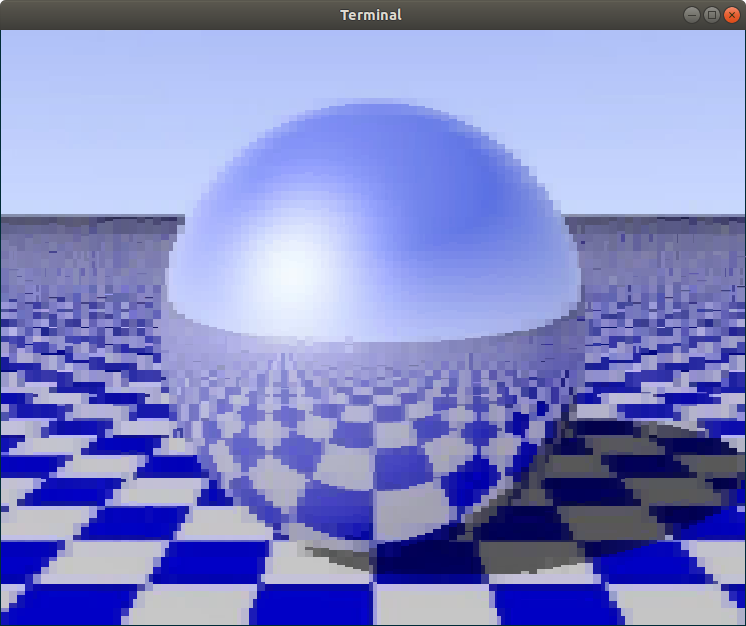
\includegraphics[width=\textwidth]{resources/checker_metal}
  \caption{Example of proposed terminal output}
  \label{fig:checker_metal}
\end{figure}

\subsection{Rendering Engines and Ray-Tracing}
\label{sec:introduction:raytracing}

A rendering engine is an algorithm that takes a scene -- a description of some space with objects -- and generates an image or visual representation of that scene.
There are many different algorithms to do this; in this proposal the recursive ray-tracing algorithm, first pioneered by Turner Whitted in his ground-breaking paper {\it An Improved Illumination Model for Shaded Display} \cite{whitted1980improved}, will be discussed and utilized.
Ray-tracing was one of the first algorithms developed in the field of computer graphics, and although there have been some improvements since then, the idea behind the algorithm is fairly straight forward.

Ray-tracing has been used as the renderer of choice for photorealistic images, since with a few modification's from Whitted's original algorithm, it can generate fantastic images.
In the past, however, it has been reserved for non-real-time uses.
For example, Figure ~\ref{fig:povray_render} is a render created by the POV-Ray engine \cite{povray}.
POV-Ray can take between a few minutes to several hours to complete one single image depending on the processing power involved.
However, there have been a few recent innovations that change this, and more details on this, as well as how ray-tracing will be utilized in \name, are discussed in Section \ref{sec:method}.

\begin{figure}[htb]
  \centering
  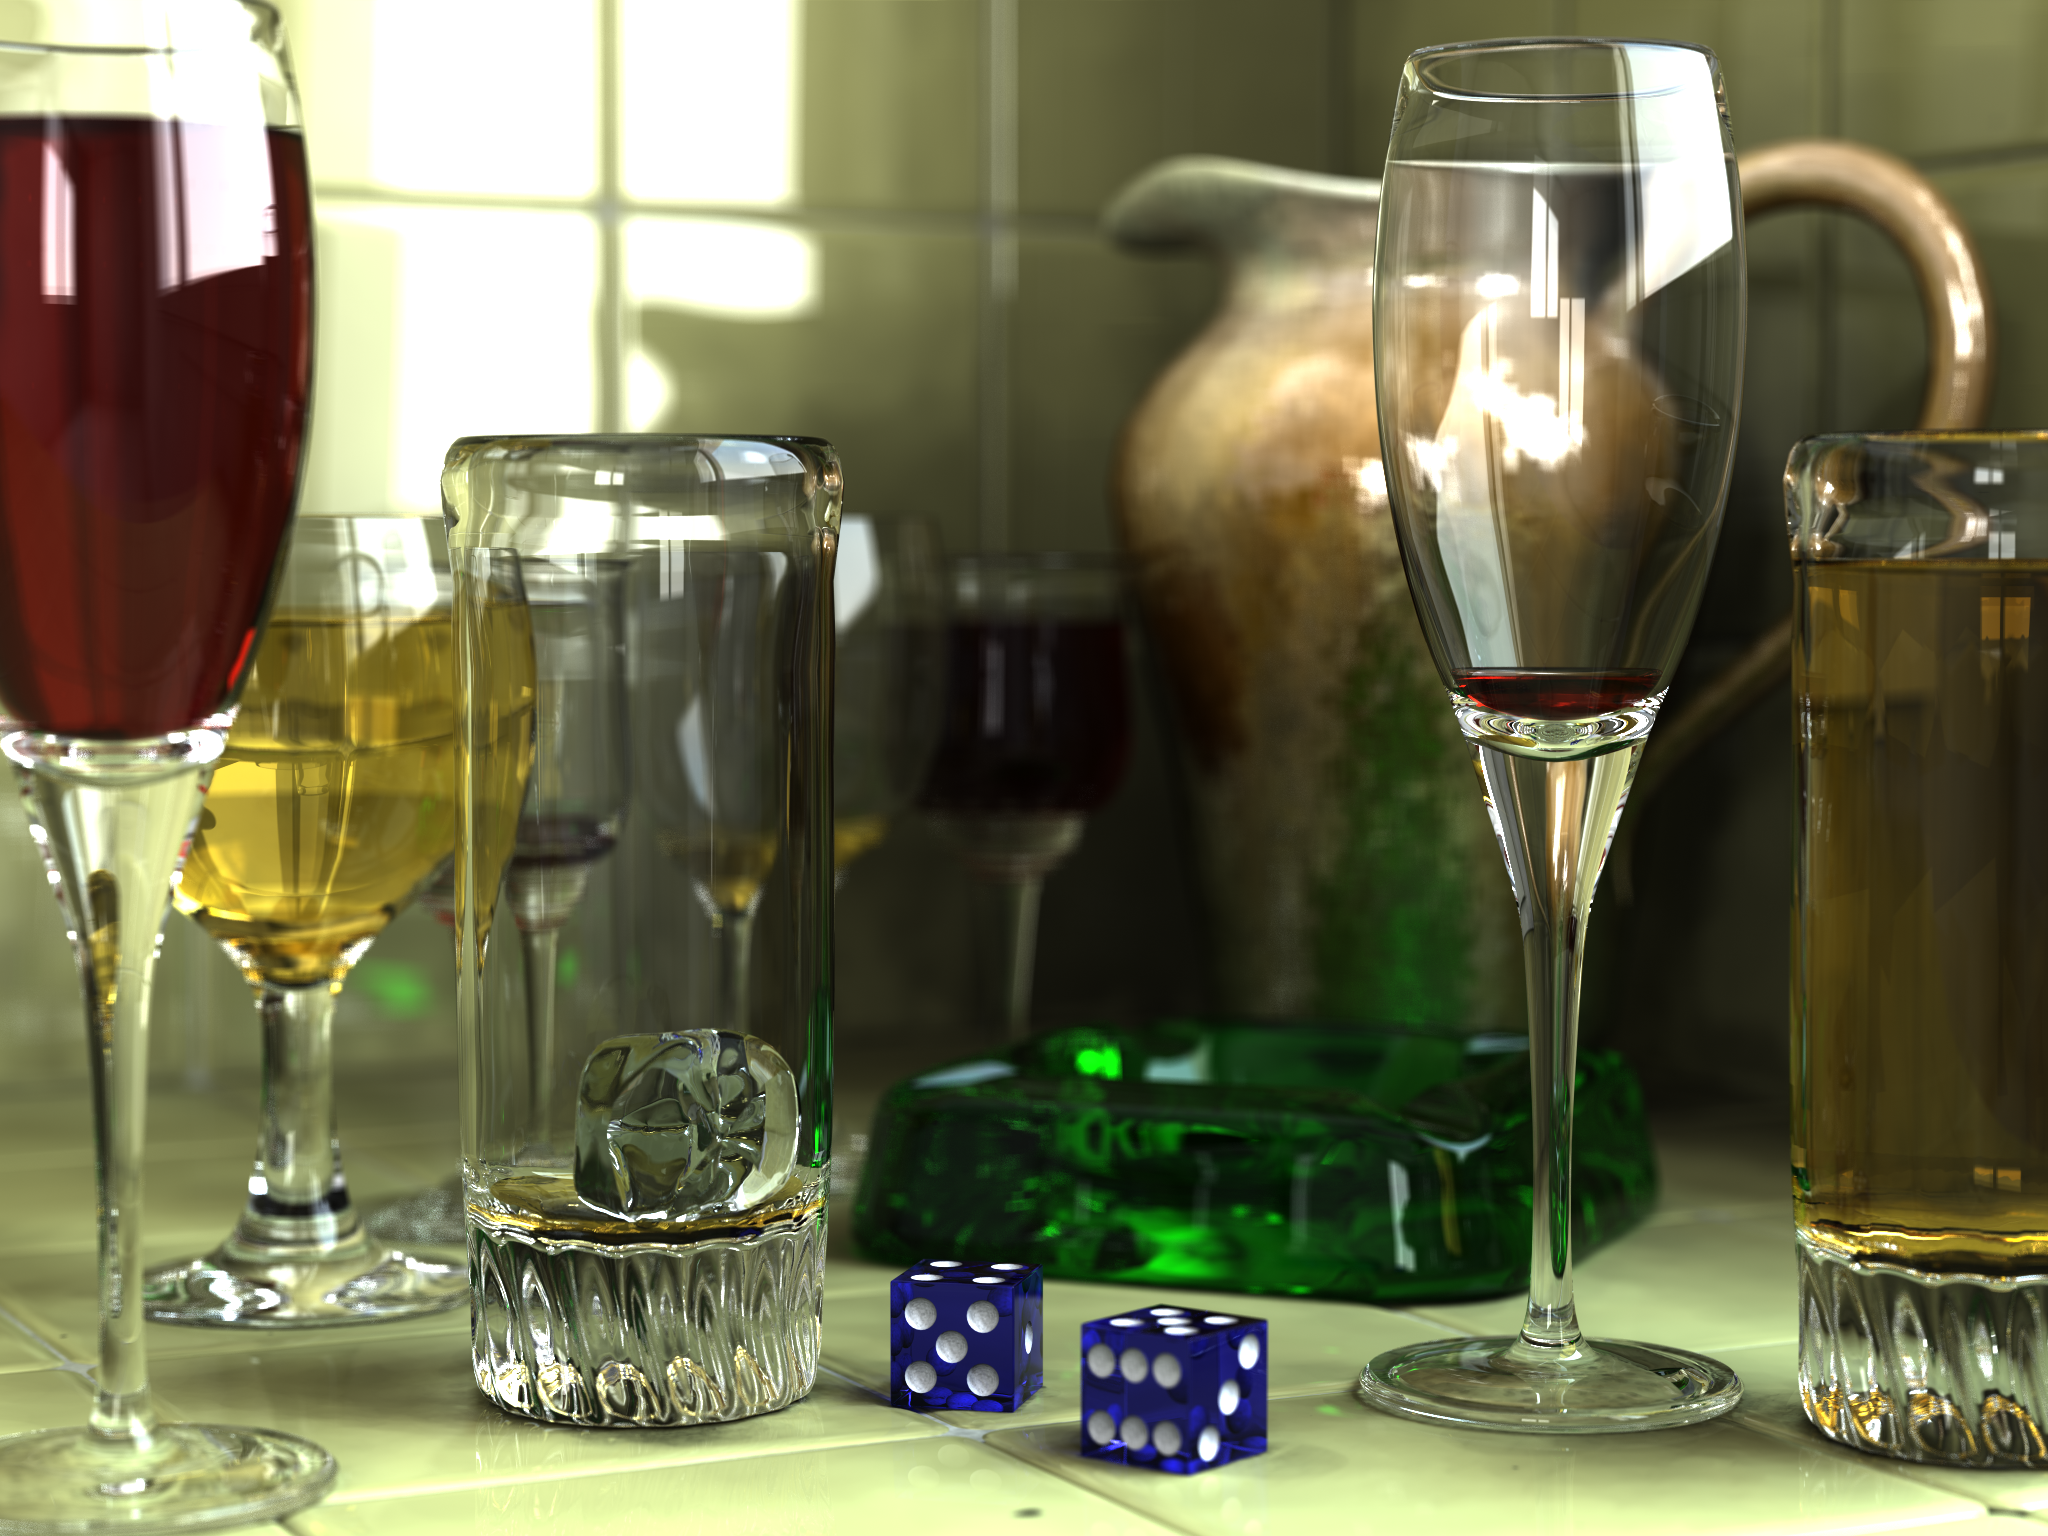
\includegraphics[width=\textwidth]{resources/glasses_povray}
  \caption{POV-Ray render created by Gilles Tran \cite{povray2006render}}
  \label{fig:povray_render}
\end{figure}


Ray-tracing revolves around the idea of {\it rays}, a mathematical construct which can be defined by two vectors: an origin point, referred to as $\rayorg$ for some ray $R$, and a direction, referenced as $\raydir$.
These two vectors together represent a ray that starts at the origin and projects along the direction; it is of infinite length.
An important addition to the concept of rays is a point along a ray -- this can be defined by using a third variable, which we will call $t$, to represent how far along the ray the point is located.
Therefore, formula ~\ref{equation:point_on_ray} can be used to get the coordinates of a point in three-dimensional space (assuming $\raydir$ is a unit vector).
This is called the {\it paramatric~form} of a ray.
The mathematics behind ray-tracing are further explored in Section ~\ref{sec:method}.

\begin{equation}
  \label{equation:point_on_ray}
  \vec{point} = \rayorg + t\raydir
\end{equation}

In ray-tracing, rays are used to simulate the path that light takes as it travels around the scene.
When a ray intersects with an object in the scene, various things can happen to simulate how light may travel under different conditions.
It is worth noting that a base assumption is made in ray-tracing when using straight rays as described here: light follows a straight line without changes.
This is only the case in reality when light travels through a vacuum with no gravitational bodies; thus basic ray-tracing is not exactly photorealistic, and does not model phenomena such as atmospheric scattering.
Additional mathematics and systems must be used to bend, attenuate, or scatter a ray to accurately render transparent volumes -- this is called volumetric ray-tracing, and will not be supported by \name, at least in the version proposed here.

The basis for ray-tracing is the rendering equation, articulated by James Kajiya in 1986 \cite{kajiya1986rendering}.
The mathematics behind the equation are covered in Section \ref{sec:method:rendering_equation}; a simplified description is that the rendering equation models the outgoing light at some point given all incoming light, a bidirectional reflectance distribution function (BDRF) and a normal for the surface at the point modeled.
If solved for every point in the scene, the rendering equation could generate a completely photorealistic image -- this would, however, require massive amounts of computation since the integral over all incoming light must be solved through numerical analysis.
Ray-tracing engines that do this are known as {\it path-tracers}, and are the most photorealistic rendering engines invented.

\name\ will not use a path-tracer -- they are still many times too slow for real-time rendering.
Instead, the rendering equation will solved by sampling the incoming light with rays.
This is known as recursive ray-tracing, since we will start with a single ray which will split every time it encounters a surface.
The eventual goal of the recursive ray-traving algorithm is to create a tree of rays for each {\it fragment} to render.
A fragment is either a pixel or some sub-pixel -- many systems will use four or more fragments per pixel to get better anti-aliasing and more accurate results.
Each ray has some color that represents the color of the light in that ray; when a ray hits an object, it is {\it scattered} by the {\it material} of the object, splitting and generating new rays.
These rays are biased towards directions that contain lots of incoming light -- such as towards a point light source.
The specific implementation of recursive ray-tracing that \name\ will use will only scatter into a set number of rays at each intersection point -- one ray toward each light source, along with reflection and refraction rays towards the relevant directions.

The base of each generated tree is a ray -- called an {\it eye-ray} -- with its origin at the camera or ``eye''.
The eye-ray's color is the color that will be rendered for that fragment.
As the eye-ray projects forward, away from the eye, it is tested for intersection with all objects in the scene.
When an intersection happens and the generated rays scattered, the eventual color values of the scattered rays are combined to produce the color of the original eye-ray.
This is done recursively to fully render the scene.


\subsection{Image Composition using Unicode Characters}
\label{sec:introduction:unicode}

Unicode is a character standard that allows anyone to reference many thousands of characters to compose text, no matter the environment around the text.
Some critical characters that \name\ will use are known as the {\it block characters} -- they are characters \texttt{U+2580} -- \texttt{U+259F}.
Contingent on the quality of the output using only block characters, additional sets could be used such as triangles and lines.
The core of image composition using Unicode is coloring the characters and the background -- \name\ will use this so that every character of the output contains two colors -- one for the background, and one for the character displayed.
This allows each {\it character~pixel} to represent a hard gradient.

There are two image modes that will be available for use in \name.
The first is pure {\it pixel mode}, in which the unicode ``half-block'' symbol is used.
Since mono-spaced character output (such as in a terminal) is twice as tall as it is wide, the half-block can split a single character into two pixels that are colored differently -- the upper pixel with the background color of the character, and the lower with the character or foreground color of the pixel.
This would mean that a typical 85 by 30 character terminal would result in a screen space of 85 by 60 pixels.
This mode also dramatically reduces the number of ray-tracing computations needed, since only one ray per pixel is required.

The second image mode is considerably more complicated and slower, as it uses significantly more rays per character in order to determine what Unicode block character most fits the desired output.
On the other hand, it allows a much higher perceived resolution, since the characters used have smaller footprints -- up to an eigth of a character in width or length.
The differences between these two modes are highlighted in Figure \ref{fig:unicode_mode_comparison1} and \ref{fig:unicode_mode_comparison2}.
It can be seen that the first image mode, {\it pixel mode}, has a rather fuzzy definition of the sphere, whereas in the second image mode, {\it block character mode}, the sphere itself, as well as the reflections seen on it, are much more defined.
The performance impact of both modes is another factor that must be assessed when choosing how to implement \name.
More details on the algorithm for ray to character translation is available in Section \ref{sec:method:ray_character_algorithm}.

\begin{figure}[htb]
  \begin{subfigure}[htb]{0.5\textwidth}
    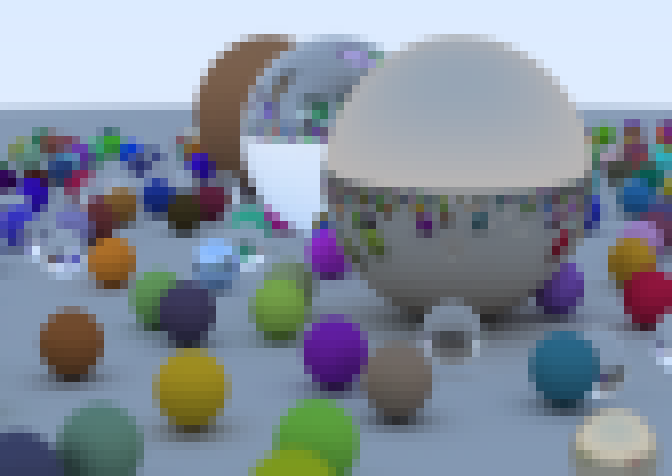
\includegraphics[width=\textwidth]{resources/many_spheres_square}
    \caption{Pixel Mode Image Output}
    \label{fig:unicode_mode_comparison1}
  \end{subfigure}
  \begin{subfigure}[htb]{0.5\textwidth}
    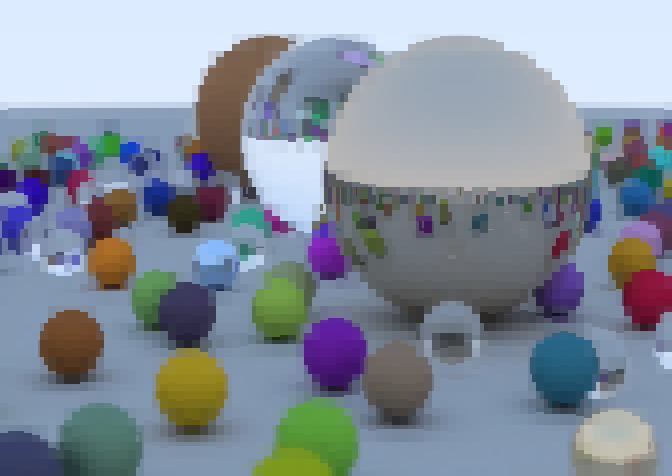
\includegraphics[width=\textwidth]{resources/many_spheres}
    \caption{Character Mode Image Output}
    \label{fig:unicode_mode_comparison2}
  \end{subfigure}
  \caption{Examples of Image Mode Output}
\end{figure}

\subsection{Terminal Output using \texttt{ncurses}}
\label{sec:introduction:ncurses}

Once an image is generated, \name\ must somehow display that image in a terminal with no surrounding prompt or other formatting -- just a simple {\it character field}.
To do this, we will use \texttt{ncurses}, a C library that abstracts implementation details of the terminal to enable full-window 24-bit color character output.
Using \texttt{ncurses}, the terminal window will be divided into two ``panels'', a main panel for the actual image output -- updated 30 to 60 times per second -- and an info panel to render information such as frames per second and logging information.
With this dependency, \name\ can be used on all terminals that support \texttt{ncurses} -- generally, any XTerm-like terminal will work, as long as it supports \texttt{termcap} or \texttt{terminfo}.

A possible limitation to \texttt{ncurses} is keyboard input handling -- it is not possible to get events on a down-movement or up-movement of a key, as is possible in some other libraries.
Therefore, some research will need to be done on possible alternatives for the input aspect of the engine.
This is, however, not a priority, since it is not related to the rendering nature of \name, and instead only helps with demonstrations of its capabilities.

\section{Related Work}
\label{sec:relatedwork}

% Summarize the previously published papers and books that are related to your
% proposed research. Whenever possible, you should compare and contrast your
% approach with the ones that have been discussed in the past. As you describe
% related papers, please make sure that you cite them
% properly~\cite{conrad-gecco-selection-study}.

% To create an image, a ray-tracer first generates {\it eye-rays}, one for each pixel to render.
% These rays have their origin at the camera, and a direction which causes the ray to pass through the pixel to render.
% Each ray is then tested against all objects in the scene for intersection, and the intersection with the closest distance is chosen.
% This was the only thing the original ray-traced shading algorithm \cite{appel1968some} did, after which the amount of illuminance incident on the point the ray hit, along with some information available from other algorithms (such as if the surface faced a light), dictated the level of darkness of that pixel.

\todo{
paragraphs for:\\
first ray tracing\\
early reverse ray tracing\\
whitted\\
the rendering equation?\\
acceleration structure\\
distributed ray tracing\\
stable ray tracing?\\
TerminalImageViewer\\
termloop\\
}

% rewrite above (use stuff on doc) and continue thread three

\section{Method of Approach}
\label{sec:method}

% Use technical diagrams, equations, algorithms, and paragraphs of text to
% describe the research that you intend to complete. See the \LaTeX\ source file
% for the proposal to learn how Figure~~\ref{intro-fig1} and Table~~\ref{intro-tab1}
% were included. Be sure to number all figures and tables and to explicitly refer
% to them in your text.


There are a lot of unsolved technical issues that will be encountered as work continues for \name.
Much of this is related to the performance and testing aspects of \name, since a high level of optimization is needed in order to obtain real-time results.
Only recently has ray-tracing even been able to achieve real-time levels of performance -- much of this progress is thanks to advances in GPU technology.
The largest innovator in this space, GPU chip design company NVIDIA, released its RTX series of GPUs that have hardware support for ray-tracing.
However, although fascinating, this proposal will not focus on RTX hardware, since its spread is slow due to the high barrier to entry because of cost.

The main technical research will be done on the OptiX API \cite{parker2010optix} for older NVIDIA GPUs that enables GPU-accelerated ray-object intersection calculations.
The main goals of this forray are to understand and use the technologies already available for non-real-time ray-tracing to do real-time work.
Although a CPU-only ray-tracer is completely possible, and likely the first step in embarking on the creation of \name, it is not likely to be performant enough for real-time graphics.
Therefore leveraging either CUDA (a compute API for NVIDIA GPUs \cite{nvidia2011cuda}) directly, or utilizing OptiX will be required.
Using a GPU is essential in this area since ray-tracing is highly parrallelizable, and can have massive speed gains from using many hundreds of cores.

The other technical challenges we cover in this section are the the mathematical basis for ray-tracing, along with details about the proposed implementation.
Much of the math is informed by Peter Shirley's excellect {\it Ray Tracing in One Weekend} \cite{shirley2016ray}, as well as the Morgan Kaufmann textbook {\it Physically Based Rendering: From Theory to Implementation} \cite{pharr2016physically}.


\subsection{Ray-Surface Intersection}

Scenes that can be ray-traced must be a collection of surfaces that are mathematically intersectable with a ray.
Any surface that can be defined by $f(\vec{p}) = 0$, that is, $f(\vec{p})$ is $0$ when $\vec{p}$ is on the surface, is intersectable with a ray.
The point of intersection can be found by solving equation ~\ref{equation:ray_surface_intersection} for $t$ and then using formula ~\ref{equation:point_on_ray} to calculate the coordinates of that point on the ray.

\begin{equation}
  \label{equation:ray_surface_intersection}
  f(\rayorg + t\raydir) = 0
\end{equation}

In \name, the only surfaces that will be supported are spheres, triangles, and infinite planes, since their surface definition functions are mathematically simple.
If there is additional development time and resources available, other shapes such as quads, abitrary polygons, and cubes may be considered.
A sphere is the simplest object to calculate ray intersection with, and therefore was the first implemented for \name.
In fact, during feasability testing the math described below was already implemented in the Go programming language.
The surface definition function of a sphere is function ~\ref{equation:sphere_surface}, with $S$ representing the sphere.
The intersection point between a ray and a sphere is given by solving equation ~\ref{equation:ray_sphere_intersection} for $t$ and then using formula ~\ref{equation:point_on_ray}.
Notice that equation ~\ref{equation:ray_sphere_intersection} is quadratic, and the number (and values) of the roots give us the $t$ we want to use.
The smallest positive root corresponds to the point on the ray which first intersects the sphere.
If there are no real roots, then the ray does not intersect the sphere.

\begin{equation}
  \label{equation:sphere_surface}
  f(\vec{p}) = (\vec{p} - \vec{S_{center}})^2 - {S_{radius}}^2
\end{equation}

\begin{equation}
  \label{equation:ray_sphere_intersection}
  (\raydir^2)t^2 + 2(\raydir \cdot (\rayorg - \vec{S_{center}}))t + (\rayorg - \vec{S_{center}})^2 - {S_{radius}}^2 = 0
\end{equation}

For planes, the surface definition function is function ~\ref{equation:plane_surface}, with $P$ representing the plane.
The plane's {\it offset} is a point on the plane, and the plane's {\it normal} is a vector perpendicular to the plane.
The intersection point between a ray and a plane is given by solving equation ~\ref{equation:ray_plane_intersection} for $t$ and then using formula ~\ref{equation:point_on_ray}.

\begin{equation}
  \label{equation:plane_surface}
  f(\vec{p}) = (\vec{p} - \vec{P_{offset}}) \cdot \vec{P_{normal}}
\end{equation}

\begin{equation}
  \label{equation:ray_plane_intersection}
  (\vec{P_{normal}} \cdot \raydir)t + \vec{P_{normal}} \cdot (\rayorg - \vec{P_{offset}}) = 0
\end{equation}

%%%%%%%% {{ description of crossing-number algorithm (not used -- too complicated, likely not optimized) }}
% The method for testing intersection with triangles is a bit more complicated, but similar to tests for other polygons.
% First, intersection is tested with the plane the triangle lies in -- this results in a ray-plane intersection point $\vec{Q}$, or no intersection.
% Then, another test must be performed if there was an intersection to detect if $\vec{Q}$ is inside the triangle.
% Before we do this we must transform our coordinate system to 2D by projecting $\vec{Q}$ and the triangle's vertices  onto the plane.
% We can define our $\vec{X}$ and $\vec{Y}$ axes to be $\vec{X} = \vec{V_0} - \vec{V_1}$ and $\vec{Y} = \vec{P_{normal}} \times \vec{X}$; our origin we define to be $\vec{Q}$.
% Finally, we can use function \ref{equation:3d_to_2d} to transform a three dimensional vector to a two-dimensional point on the plane.
%
% \begin{equation}
%   \label{equation:3d_to_2d}
%   f(\vec{w}) = [(\vec{w} - \vec{Q}) \cdot \vec{X},\ (\vec{w} - \vec{Q}) \cdot \vec{Y}]
% \end{equation}
%
% After converting our triangle vertices $\vec{V_0}, \vec{V_1}, \vec{V_2}$ to planar coordinates, we can test whether the triangle defined by them includes the origin $\vec{Q}$.
% We will do this using the ``crossing number'' method; first, create an arbitrary 2D ray with $\rayorg = [0, 0]$ and $\raydir = [0,\ 1]$.
% Then, we will use equation \ref{equation:ray_line_intersection} -- the  ray-line intersection test -- to test each edge of the triangle to see if it intersects.
% If it does, we add one to the crossing number; then, after testing every edge of the triangle, if the crossing number is even $\vec{Q}$ is outside the triangle.
% Otherwise, $\vec{Q}$ is inside the triangle.

The method for testing intersection with triangles is a bit more complicated, but similar to tests for other polygons.
The mathematics for this section are heavily modified and adapted from Jean-Colas Prunier's Scratchapixel, an excellent and accessible online resource for 3D rendering \cite{prunier2017triangle}.
First, intersection is tested with the plane the triangle lies in -- this results in a ray-plane intersection point $\vec{Q}$, or no intersection.
Then, another test must be performed, if there was an intersection, to detect if $\vec{Q}$ is inside the triangle.
We will do this using the ``inside-outside'' method: test if $\vec{Q}$ is on the left side of each edge.
First, we label each triangle vertex $\vec{V_i}$, with $i$ increasing in the counter-clockwise direction.
Then we can use function \ref{equation:left_edge_test}; if $f(i) > 0$ for each $i$, then $\vec{Q}$ is inside.
Otherwise, $\vec{Q}$ is outside the triangle
.Note that in function \ref{equation:left_edge_test}, if $i = 3$, then $i = 0$ ($i$ ``wraps'' to only valid values) Additionally, this method will work for for any $n$-sided convex polygon (such as rectangles).

\begin{equation}
  \label{equation:left_edge_test}
  f(i) = P_{normal} \cdot ((\vec{V_{i+1}} - \vec{V_i}) \times (\vec{Q} - \vec{V_i}))
\end{equation}

Function \ref{equation:left_edge_test} can be complicated to visualize, so imagine this: we first form two vectors, both with $\rayorg = \vec{V_i}$.
One points along the triangle's edge, while the other points to $\vec{Q}$.
Both of these vectors will be in the plane of the triangle.
Thus, if we cross them, the vector produced will either be away from the plane in the same direction as $\vec{P_{normal}}$, or away from the plane in the opposite direction.
According to the right hand rule, if the crossed vector is in the same direction as $\vec{P_{normal}}$, then the vector pointing to $\vec{Q}$ is ``to the left'' of the vector pointing towards $\vec{V_{i+1}}$.
We can then get the dot product between $\vec{P_{normal}}$ and the crossed vector -- if it is positive then the crossed vector is in the same direction as the normal, and therefore $\vec{Q}$ is to the left of the edge.
One last addendum to this intersection test is the the fact that it is very difficult to perform the counter-clockwise numbering of vertices -- therefore, we will simply expect vertices to be specified in counter-clockwise order.
This is similar to what many other 3D rendering programs assume.

\subsection{Rendering Equation}
\label{sec:method:rendering_equation}
Equation \ref{equation:rendering} is a slightly simplified form of the rendering equation, removing properties dealing with the wavelength of light and time.

\begin{equation}
  \label{equation:rendering}
  L_{out}(\vec{x}, \vec{w}) = L_{emit}(\vec{x}, \vec{w}) + \int_{\Omega} f_r(\vec{x}, \vec{v},\vec{w})f_i(\vec{x}, \vec{v})(-\vec{v} \cdot n) dv
\end{equation}

\todo{complete equation explanation}

\subsection{Real-time Demonstrations}
\label{sec:method:realtime_demo}

Details on the individual scenes planned are given in Section \ref{sec:evaluate}.

\todo{write technical description of implementations for camera movement, scene loading, etc}

\subsection{Ray-Character Translation Algorithm}
\label{sec:method:ray_character_algorithm}

To translate the color result of a ray-trace to an actual character pixel, a similarity test is used.
This algorithm is loosely inspired by the pixel to character translation algorithm used in TerminalImageViewer \cite{tivGithub}; however, it has less input data -- instead of a 4 by 8 pixel field, only a few color samples from ray-tracing results are available.

\todo{complete algorithm description}

\section{Discussion}
\label{sec:discussion}

\todo{introduce discussion section -- how?}

\subsection{Evaluation}
\label{sec:evaluate}

% Explain what steps you will take to evaluate your proposed method. If you intend
% to conduct experiments, then you must clearly define your evaluation metrics.

The first step in evaluating a ray-tracer is to get the output in an easily compared form -- for \name, a debug mode called {\it \texttt{ppm} mode} will generate image files in portable pixmap format.
This mode will be a different interface in addition to the \texttt{ncurses} character output modes, allowing much higher resolution output for testing.
It is unlikely that this will be real-time capable, but render times for \texttt{ppm} images with millions of fragments will serve as good benchmarks for algorithm optimizations.
The image format \texttt{ppm} was chosen for it's human readability along with ease of use for development -- it has both ASCII and binary forms, with the ASCII being more useful in our case.
The format is extremely simple; a \texttt{ppm} file is shown in Figure \ref{fig:ppm_code}, with Figure \ref{fig:ppm_image} being its output.

\begin{figure}[htb]
  \begin{subfigure}[htb]{0.5\textwidth}
    \small
    \begin{verbatim}
      P3 # header
      3 2 # width x height
      255 # max color value
      # image data -- RGB triplets
      # (extra whitespace is ignored)
      255   0   0     0 255   0
        0   0 255   255 255   0
      255 255 255     0   0   0
    \end{verbatim}
    \caption{Example \texttt{ppm} file contents}
    \label{fig:ppm_code}
  \end{subfigure}
  \begin{subfigure}[htb]{0.5\textwidth}
    
\includegraphics[width=\textwidth]{resources/ppm_example}
    \caption{Example \texttt{ppm} image}
    \label{fig:ppm_image}
  \end{subfigure}
  \caption{Portable pixmap format example}
\end{figure}

Using this \texttt{ppm} image output mode will enable graphical quality comparisons, testing, and bug-fixing.
It can also provide output and results data for easily implemented regression testing, to ensure any changes are purposeful.
Lastly, the \texttt{ppm} mode can be used to test the fidelity of \name's ray to character translation algorithm against other available algorithms in programs such as TerminalImageViewer by providing a single, identical input image for translation.

In addition to the \texttt{ppm} mode, demonstration scenes will also be built to enable real-time testing of the ray-tracing algorithm and \name's associated systems.
These scenes will essentially act as integration tests, as well as provide demonstrations of \name's capabilities.
The final project will include at least the following scenes, but may be more extensive.

\begin{itemize}
  \setlength\itemsep{-0.25em}
  \item Whitted's Sphere
  \item Cornell's Box
  \item Shadow Demo
  \item Moving Object
  \item Environment Exploration
\end{itemize}

The first two scenes are famous ray-tracing example scenes, and can be used to benchmark the performance of \name\ against other ray-tracing engines such as Octane or Blender.
The other three are demo scenes designed to showcase certain aspects of \name.
The Shadow Demo scene is a simple scene similar to NVIDIA's RTX shadow demo, seen in Figure \ref{fig:nvidia_shadows}.
It demonstrates soft shadows, and will show the limitations of \name's ray-tracer, since at least at the moment only point lights will be supported.
When this scene is implemented, and if there is time in the development schedule, area lights may be implemented through multiple random sampling.
This simple addition to recursive ray-tracing simply adds more shadow rays to each scatter, randomly spread between any area lights in the scene.

\begin{figure}[htb]
  \centering
  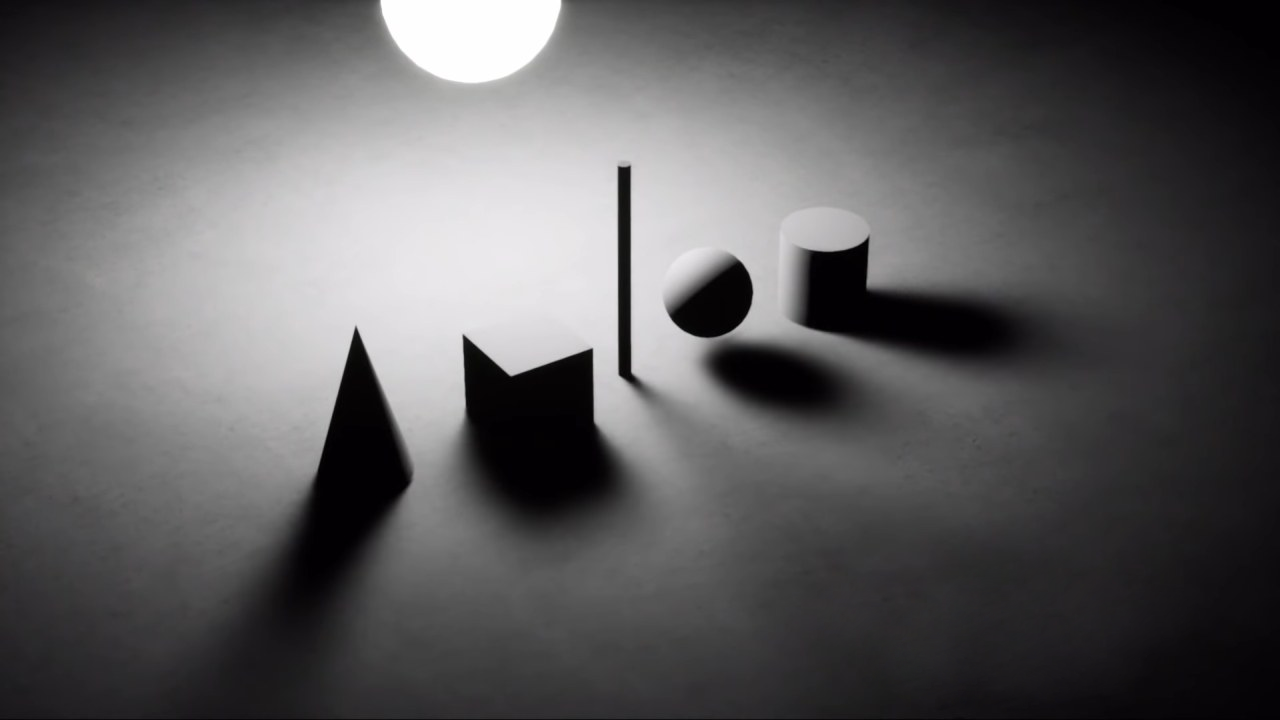
\includegraphics[width=\textwidth]{resources/nvidia_shadows}
  \caption{NVIDIA Shadow Scene -- shown at CES 2018, NVIDIA Keynote}
  \label{fig:nvidia_shadows}
\end{figure}

The Moving Object scene will be modeled after a typical Cornell Box, however the main point of the scene will be object and light source movement -- animated in real time.
This will stress the ray-tracer and demonstrate the real-time shadows, lighting, and rendering to the fullest extent.
Finally, the Environment Exploration scene is a somewhat nebulous idea -- it is a scene where the user can ``explore'' and move the camera around to experience a wider area.
Currently envisioned as a set of complex models of a street corner or otherwise realistic location, it will be the stress test for \name.
As many thousands of objects and possibly millions of rays are computed per second, this scene will ensure the ray-tracing algorithm is well-designed and optimized.

Along side the scene demonstrations will also be material demonstrations -- although simple in nature, they will show off the different implementations of lambertian, dielectric, and metal materials, along with other possible effects such as glass, tessellation, and ray-traced bump mapping.
Many of these effects are contingent upon available development time, however at least a few should be available in the final project.

\subsection{Development Schedule}
\label{sec:schedule}

% Identify the main phases and tasks of your research project and set deadlines
% for when you will be able to complete each of these items.

Table \ref{worktable} proposes a schedule for the implementation and research work needed to complete \name.
First, a CPU implementation of the recursive ray-tracing algorithm would be developed, at first tested in \texttt{ppm} output mode.
Then, as the ray-tracing code grows to a testable state, the interface to ncurses would be developed.
This involves implementing the ray to character translation algorithm, as well as standardizing an interface with which another render engine (specifically the future GPU ray-tracer) can interface with the displayed terminal image.

\begin{table}[htb]
  \vspace*{0.6em}
  \centering
  \begin{tabular}{|c||c|c|}
    \hline
    \textbf{Task} & \textbf{Begin Date} & \textbf{End Date} \\\hline\hline
    Proposal defense prep & Early Nov & Mid Nov \\\hline
    CPU ray-tracer impl & Late Nov & Early Jan \\\hline
    \texttt{ncurses} interface impl & Mid Dec & Late Jan \\\hline
    OptiX/CUDA research & Mid Dec & Early Jan \\\hline
    Thesis chapter outlines & Early Dec & Late Jan \\\hline
    GPU impl/rewrite & Early Jan & Early Feb \\\hline
    Scene/material creation & Mid Dec & Late Mar \\\hline
    Thesis chapter writing & Early Feb & Early April \\\hline
    Graphics Testing & Early Mar & Mid Mar \\\hline
    Thesis defense prep & Early Apr & Mid Apr \\\hline
  \end{tabular}
  \caption{Proposed work schedule}
  \label{worktable}
\end{table}

Once both the CPU ray-tracer and \texttt{ncurses} implementations are nearing completion, research will begin on OptiX/CUDA integration.
The design and architecture of the GPU ray-tracer will take the lessons learned in the implementation of the CPU ray-tracer and use them to improve organization and understandability.
Additionally, the GPU ray-tracer will be highly parallel, and so extra care must be taken to avoid the problems that are involved with parallelization.
As the design phase for the GPU ray-tracer is wrapping up, thesis writing will commence.
The first stages will document the challenges and lessons learned from completing the CPU ray-tracer, including performance testing and evaluation.
Additional thesis outlines will be generated to guide work on the final GPU ray-tracer.

Finally, implementation of \name's actual GPU ray-tracing engine will begin in early January.
From this point onward, implementation and demonstration will be the primary goals.
By late February final demonstration scene creation should be wrapping up, and materials should be well on their way to completion.
Thesis chapter writing begins in earnest, with disscussions of the various new GPU-based techniques used for the GPU ray-tracer the primary focus.
Finally, end result testing and graphical comparisons will be made, along with preparation for the thesis defense.

\section{Conclusion}
\label{sec:conclusion}

% Provide a summary of your proposed research and suggest the impact that it may
% have on the discipline of computer science. If possible, you may also suggest
% some areas for future research.

\todo{write conclusion}


\bibliographystyle{plain}
\bibliography{senior_thesis_proposal}
\end{document}
